\documentclass[]{beamer}
%\usepackage[utf8]{inputenc}
%\usepackage{amsmath}
\usepackage{pgfplots}
\usetheme{Singapore}
\usefonttheme{serif}
\usecolortheme{lily}
\title{Introduction to Derivative Pricing:}
\subtitle{An intro to Baxter \& Rennie}
\author{guoxiaoq@gmail.com}
\date{}
\begin{document}
\section{Betting Game}
\begin{frame}
  \titlepage
\end{frame}
\frame{\frametitle{Horse Gambling Example}
  \begin{itemize}
  \item Horse A has a 25\% chance of winning the race, B has 75\% \pause
  \item On the market there are \$5000 betting for A, and \$10000 betting for B. \pause
  \item How should the book maker set the odds for A and B assuming no margin? \pause
  \item Using the market supply and demand, his profit is not dependent on the actual outcome. \pause
  \item Using the actual probability, his short-term PnL will be dependent on the race outcome \pause
  \item so how should he decide on the odds? 
  \end{itemize}
}
\frame{\frametitle{Power of Arbitrage}
  As seen from the house gambling example, arbitrage is a better pricer than expectation. Financial instrument pricing is determined in the same way. \pause
  \begin{itemize}
  \item Arbitrage opportunity would be a (self-financing) trading strategy which started with zero value and terminated at some definite date T with a positive value.
  \item How do you price the share of Apple?
    \pause  
  \item How do you price the call option on Apple share? 
    \pause
  \item How to price 1 million Apple shares? 
  \end{itemize}
}

\frame{\frametitle{No Arbitrage Pricing}
  \begin{itemize}
  \item No-arbitragee implies no way of making riskfree profits. \pause
  \item Arbitrage is a stronger pricing argument than expectation. \pause
  \item Arbitrage activity in the market will drive price to no-arb pricing. 
  \end{itemize}
}

\frame{\frametitle{ Betting/Trading strategy}
  What are the elements that goes into a betting/trading strategy? 
  \begin{itemize}
  \item instrument/Rule: what to bet. What are the possible outcomes that would be known later.
  \item quantity: how much to bet.
  \item odds/market price:  What are the payoffs for the pay for each possible outcome?
  \item Rule:pre-visibility: Bets off before the outcome is known. No cheating
  \end{itemize}
}

\frame{\frametitle{Martingale: double down stragetgy}
  For a fair coin toss ( odds at 1:1 ) bet, bet \$1 for head, and double the bet each time tails shows until the 1st head shows. This will give you a sure profit of \$1, as long as you don't go broke before the 1st heads shows.
  \begin{itemize}
  \item Can it be carried out in Marina Bay Sands?
  \item Why martingale is not an arbitrage? \pause --- not self-financing
  \end{itemize}
}

\section{Binonmial}
\frame{\frametitle{Binomial representation theorem (I)}
  \begin{itemize}
  \item A random process is described using binomial tree nodes for all possible future values.
  \item A probability set for the above tree, called measure.
  \item Filtration $\mathcal{F}_i$ is the historical path upto $i$. This can be seen as information set available up to time $i$.
  \item Claim $X$ is a function depends on $\mathcal{F}_T$.
  \item $\mathbb{E_Q}(X|\mathcal{F}_i)$, converts a claim into a process, i.e. price of the claim at each $t$.
  \item A previsible process/trading stragegy
  \item A martingale measure. ( $\mathbb{E_P}(S_j|\mathcal{F}_i)=S_i$, for all $i \leq j$. )
  \end{itemize}
}

\frame{\frametitle{Binomial representation theorem (II)}
  \begin{theorem}
    Suppose the measure Q is such that the binomial price process S is a Q-martingale. If N is any other Q-martingale, then there exists a previsible process h such that \[ N_i = N_0 + \sum_{k=1}^i h_k \Delta S_k ,\] where $\Delta S_k := S_i - S_{i-1}$ is the change in $S$ from time $i-1$ to $i$, and $h_i$ is the value of $h$ at the appropriate node at time $i$. 
  \end{theorem}
}\frame{\frametitle{Binomial representation theorem (III)}
  \begin{itemize}
  \item As a result, all claimes can be fully replicated using simple trading strategies and therefore strongly priced by no-arbitrage argument. This is also called market completeness.
  \item arbitrage free = market complete = existence of unique Equivalence of Martingale Measure
  \item The theorem can be extended to continuous-time version.
  \end{itemize}
}
\section{Martingale}
\frame{\frametitle{Brownian motion}
  \begin{definition}
    The process $W = (W_t : t \geq 0)$ is a $\mathbb{P}$-Brownian motion if and only if:
    \begin{enumerate}
    \item $W_t$ is continuous, and $W_0$ = 0,
    \item the value of $W_t$ is distributed, under $\mathbb{P}$, as a normal random variable $N(0,t)$
    \item the increment $W_{s+t} - W_s$ is distributed as a normal $N(0,t)$, under $\mathbb{P}$, and is independent of $\mathcal{F}_s$, the history of what the process did up to time $s$.
    \end{enumerate}
  \end{definition}
}
\frame{\frametitle{Stochastic process}
  \begin{definition}
    A stochastic process $X$ is a continous process ( $X_t:t\geq0$) such that $X_t$ can be written as \[ X_t = X_0 + \int_0^t \sigma_s dW_s + \int_0^t\mu_sds,\] where $\sigma$ and $\mu$ are random $\mathcal{F}$-previsible process such that $\int_0^t(\sigma_s^2+|\mu_s|)ds$ is finite for all times $t$ (with probability 1 ). The differential form of this equation can be written \[dX_t=\sigma_tdW_t+\mu_tdt.\]
  \end{definition}
}
\frame{\frametitle{It$\hat{\textrm{o}}$'s formula}
  If $X$ is a stochastic process, satisfying $dX_t=\sigma_tdW+\mu_tdt,$ and $f$ is a deterministic twice continously differentiable function, then $Y_t:=f(X_t)$ is also a stochastic process and is given by \[dY_t=\left(\sigma_tf'(X_t)\right)dW_t+\left(\mu_tf'(X_t)+\frac{1}{2}
  \sigma_t^2f''(X_t)\right)dt.\]
  \begin{example}
    If $X_t = \exp(\sigma W_t)$, then what is $dX_t$?
    \pause
    \[dX_t=\sigma X_tdW_t+\frac{1}{2}\sigma^2X_tdt.\]
  \end{example}
} 
\frame{\frametitle{Radon-Nikodym derivative}
  \begin{definition}
    \emph{Equivalence} \\
    Two measures P and Q are equivalent if they operate on the same sample space and agree on what is possible. \[P(A)>0 \Leftrightarrow Q(A) > 0.\]
  \end{definition}
  \begin{definition}
    Given $\mathbb{P}$ and $\mathbb{Q}$ equivalent measures and a time horizon T, we can define a random variable $\frac{d\mathbb{Q}}{d\mathbb{P}}$ defined on $\mathbb{P}$-possible paths, taking positive real values, such that
    \begin{enumerate}
    \item $\mathbb{E_Q}(X_T)=\mathbb{E_P}(\frac{d\mathbb{Q}}{d\mathbb{P}}X_T),$ for all claims $X_T$ knowable by time $T$.
    \item $\mathbb{E_Q}(X_t| \mathcal{F}_s) = \xi_s^{-1}\mathbb{E_P}(\xi_t X_t|\mathcal{F}_s), \ s\leq t \leq T,$
    \end{enumerate}
    where $\xi_t$ is the process $\mathbb{E_P}(\frac{d\mathbb{Q}}{d\mathbb{P}}|\mathcal{F}_t).$
  \end{definition}
}
\frame{\frametitle{Cameron-Martin-Girsanov theorem}
  \begin{theorem}
    If $W_t$ is a $\mathbb{P}$-Brownian motion and $\gamma_t$ is a $\mathcal{F}$-previsible process satisfying the boundedness condition $\mathbb{E_P}\exp(\frac{1}{2}\int_0^T\gamma^2_tdt)<\infty$, then there exists a measure $\mathbb{Q}$ such that 
    \begin{enumerate}
    \item $\mathbb{Q}$ is equivalent to $\mathbb{P}$
    \item $\frac{d\mathbb{Q}}{d\mathbb{P}}=\exp\left( - \int_0^T \gamma_tdW_t - \frac{1}{2}\int_0^T\gamma^2_tdt\right)$
    \item $\widetilde{W}_t = W_t + \int_0^t\gamma_sds$ is a $\mathbb{Q}$-Brownian motion.
    \end{enumerate}
    In other words, $W_t$ is a drifting $\mathbb{Q}$-Brownian motion with drift $-\gamma_t$ at time $t$.
  \end{theorem}
}
\frame{\frametitle{Martingale representation theorem}
  \begin{definition}
    A stochastic process $M_t$ is a \emph{martingale} with respect to a measure $\mathbb{P}$ if and only if
    \begin{enumerate}
    \item $\mathbb{E_P}(|M_t|)<\infty, \forall t$
    \item $\mathbb{E_P}(M_t|\mathcal{F}_s)= M_s, \forall s \leq t.$
    \end{enumerate}
  \end{definition}
  \begin{theorem}
    Suppose that $M_t$ is a $\mathbb{Q}$-martingale process, whose volatility $\sigma_t$ satisfies the additional condition that it is (with probability one) always non-zero. Then if $N_t$ is any other $\mathbb{Q}$-martingale, there exists an $\mathcal{F}$-previsible process $\phi$ such that $\int_0^T\phi_t^2\sigma_t^2dt < \infty, a.s.$, and $N$ can be written as \[N_t=N_0+\int_0^t\phi_sdM_s.\] Further $\phi$ is (essentially) unique.
  \end{theorem}
}
\section{Application}
\frame{\frametitle{Construction of Dynamic Hedging Strategy}
  Under no-arb pricing, we can fully hedge any contigent claim using following steps:
  \begin{itemize}
  \item The Portfolio $(\phi,\psi)$, where $\phi_t$ and $\psi_t$ is the number of units of security and bond we hold at $t$. $\phi$ is $\mathcal{F}$-\emph{previsible} (in other words, left continuous).
  \item Self-financing SDE $dV_t = \phi_t dS_t + \psi_t dB_t.$
  \item Suppose we are in a market of a riskless bond $B$ and a risky security $S$ with volatility $\sigma_t$, and a claim $X$ on events up to time $T$. A \emph{replication strategy} for $X$ is a self-financing portfolio $(\phi, \psi)$ such that $\int_0^T \sigma_t^2 \phi_t^2 dt < \infty$ and $V_T = \phi_T S_T + \psi_T B_T = X.$
  \end{itemize}
}
\frame{\frametitle{Black Scholes Formula}
  We assume a bond price $B_t$ and a stock price $S_t$ that follow 
  \begin{align*}
    S_t &= S_0 \exp( \sigma W_t + \mu t) \\
    B_t &= \exp(rt)
  \end{align*}
  \begin{enumerate}
  \item Find a measure Q under which $Z_t := B_t^{-1}S_t$ is a martingale. $B_t$ is therefore the \emph{numeraire}.
  \item Find the process $E_t=\mathbb{E_Q}(B_T^{-1}X|\mathcal{F}_t).$
  \item Find a previsible process $\phi$, such that $dE_t = \phi_tdZ_t$
  \item We then have 
    \begin{align*}
      V_t &= B_t \mathbb{E_Q}(B_T^{-1}X | \mathcal{F}_t) \\
      V_0 &= e^{-rT} \mathbb{E_Q}(X)
    \end{align*}
  \end{enumerate}  
  which can be easily solved analytically.
}

\frame{\frametitle{Application to FX: assumptions}
  We assume constant interest rate for domestic and foreign currency, and the exchange rate expressed in units of domestic currency per 1 foreign currency follows GBM.
  \begin{align*}
    B_t&=e^{rt}\\
    D_t&=e^{ut}\\
    S_t&=S_0 \exp(\sigma W_t + \mu t)
  \end{align*}
  for some $W_t$ a $\mathbb{P}$-Brownian motion and constants $r$, $u$,$\sigma$, and $\mu$, where $D_t$ is the foreign cash bond.
}
\frame{\frametitle{Application to FX: approach }
  \begin{itemize}
  \item Choose the numeraire: $B_t$.
  \item Make all tradables in this numeraire a martigale at the same time.
    \begin{itemize}
    \item demostic bond becomes 1. 
    \item foreign bond is not tradable in domestic ccy
    \item fx rate itself is not a tradable
    \item foreign bond multiply by the fx spot is. $Z_t = B_t^{-1}S_t D_t$ needs to be a martingale. 
    \end{itemize}
  \item form the martigale process of the derivative value $E_t = \mathbb{E_Q}(B_T^{-1}X|\mathcal{F}_t)$.
  \item find the hedging strategy $\phi_t$, s.t. $dE_t=\phi_tdZ_t$.
  \end{itemize}
}
\frame{\frametitle{Application to FX: general formula}
  \begin{itemize}
  \item original converted foreign bond process in numeraire $B_t$: $$Z_t = S_0 \exp ( \sigma W_t + ( \mu + u - r ) t )$$
  \item we need to make it into a martingale by changing the drift: 
    $$Z_t = S_0 \exp ( \sigma \tilde{W}_t - \frac{1}{2}\sigma^2t )$$
  \item therefore the fx process becomes via the same drift change: 
    $$S_t = S_0 \exp ( \sigma \tilde{W}_t + ( r - u - \frac{1}{2}\sigma^2 ) t )$$
  \item so we have the derivative pricing formula: 
    $$V_t = B_t\mathbb{E_Q}(B_T^{-1}X|\mathcal{F}_t)$$
  \end{itemize}
}
\frame{\frametitle{Application to FX: forward }
  Let's price a forward $V_T = S_T - K$ using the formula.
  \begin{align*}
    V_t &= B_t\mathbb{E_Q}(B_T^{-1}X|\mathcal{F}_t) \\
    V_0 &= e^{-rT}(\mathbb{E_Q}(S_T) - K) \\
    V_0 &= e^{-rT}(S_0 e^{(r-u)T} - K ) \\
  \end{align*}
}
\frame{\frametitle{Application to FX: Call option}
  Let's price a call option $V_T = (S_T - K )^+$ using the formula.
  \begin{align*}
    V_t &= B_t\mathbb{E_Q}(B_T^{-1}X|\mathcal{F}_t) \\
    V_0 &= e^{-rT}(\mathbb{E_Q}(S_T - K)^+ \\
    V_0 &= e^{-rT}(F_0 N(d_1) - KN(d_2) ) \\
  \end{align*}
  Illustration of expectation of lognormal distribution: $F_T = F_0 e^{\sigma \sqrt{T} \tilde{W}_T - \frac{1}{2} \sigma^2 T}$:
  \begin{align*}
    \mathbb{E_Q}(1_{F_T>K}) &= P(F_T>K) \\ 
    &= P( F_0 e^{\sigma \sqrt{T} \tilde{W}_T - \frac{1}{2} \sigma^2 T} > K ) \\
    &= P( \tilde{W}_T > \frac{\ln{ \frac{K}{F_0}}+\frac{1}{2} \sigma^2 T}{\sigma\sqrt{T}} ) \\
    &= P( \tilde{W}_T < \frac{\ln{ \frac{F_0}{K}}-\frac{1}{2} \sigma^2 T}{\sigma\sqrt{T}} )  = N(d_2)
  \end{align*}
}
\frame{\frametitle{Application to FX: view from foreign side }
  Let's price a put option from the foreign investor point of view. A call on 1 EUR for 1.25 USD should be the same as 1.25 put on 1 USD for 0.8 EUR. Assuming spot and forward are all 1, and interest rates are all 0. We have
  \begin{align*}
    C &= F N(d_1) - K N(d_2) = N(d_1) - 1.25 N( d_2) \\
    1.25 \tilde{P} &= 1.25 (\tilde{K} N(-\tilde{d_2}) - \tilde{F}N(-\tilde{d_1})) = N(-\tilde{d_2}) - 1.25 N(-\tilde{d_1})\\
    d_1 &= \frac{\ln{\frac{F}{K}}+\frac{1}{2}\sigma^2T}{\sigma \sqrt T} = \frac{\ln{0.8}+\frac{1}{2}\sigma^2T}{\sigma \sqrt T} = -\frac{\ln{1.25}-\frac{1}{2}\sigma^2T}{\sigma \sqrt T} = - \tilde{d_2}\\
  \end{align*} 
  Whether we use domestic measure or foreign one, the pricing and hedging is consistent.
}
\frame{\frametitle{Application to Quantos: Assumptions}
  Assuming a foreign asset, and fx process both follow lognormal process, with constant interest rates.
  \begin{align*}
    dS_t &= \mu S_t d_t+ \sigma_1 S_t dW_1(t) \\
    dC_t &= v C_t d_t + \sigma_2 C_t dW_2(t)
  \end{align*}
  $dW_1$ and $dW_2$ is correlated at $\rho$.
}
\frame{\frametitle{Application to Quantos: Numeraire and tradables}
  \begin{itemize}
  \item $B_t$, numeraire.
  \item $C_t D_t$, dollar tradable of foreign bond
  \item $C_t S_t$, dollar tradable of foreign asset
  \end{itemize}
  We need to do a change of measure so that all of the tradables are martingales
  \begin{align*}
    Y_t &= B_t^{-1}C_tD_t \\
    Z_t &= B_t^{-1}C_tS_t
  \end{align*}
}
\frame{\frametitle{Application to Quantos: formula }
  The result of the change is expected: fx process same as the fx option case, quantoed asset process just change the drift, due to correlation to fx process. 
  \begin{align*}
    dS_t &= ( u - \rho\sigma_1\sigma_2 ) S_t d_t+ \sigma_1 S_t d\tilde{W}_1(t) \\
    dC_t &= ( r - u ) C_t d_t + \sigma_2 C_t d\tilde{W}_2(t)
  \end{align*}
  The pricing formula is as usual: $$V_t = B_t\mathbb{E_Q}(B_T^{-1}X|\mathcal{F}_t),$$ where $X$ is a function of $S_T$ like a forward or call. 
}
\frame{\frametitle{Application to Composite}
  \begin{itemize}
  \item What is the tradable?
  \item What is the process? 
  \item Using a single composite process with a simple payoff generates the same answer as using the quanto processes with a composite payoff 
  \end{itemize}
}
\section{Term Structure}
\frame{\frametitle{Application to Interest Rate}
  \begin{enumerate}
  \item [$P(t,T)$] discount bond price with maturity $T$ at $t$ 
  \item [$R(t,T)$] bond yield ( continuous compounding ). $R(t,T) = -\frac{\ln P(t,T)}{T-t}$

    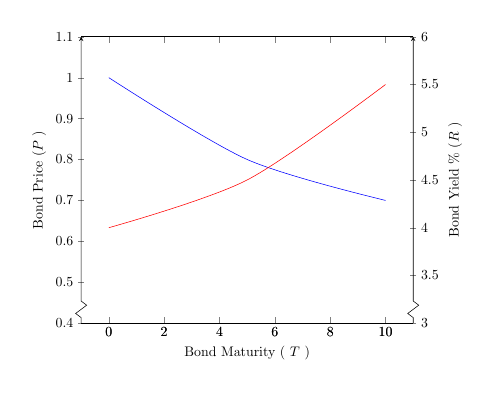
\begin{tikzpicture}[scale = 0.5]
      \begin{axis}[
	  scale only axis,
	  axis y line=left,
	  ymin=.4,
	  ymax = 1.1,
	  axis y discontinuity=crunch,
	  xlabel = Bond Maturity ( $T$ ),
	  ylabel = Bond Price ($P$ )]
        \addplot+[smooth, no marks] 
	plot coordinates{ 
	  (0,1) 
	  ( 5, .8 ) 
	  ( 10, .7 )
	};
      \end{axis}		
      \begin{axis}[
	  scale only axis,
	  axis y line=right,
	  ymin=3,
	  ymax = 6,
	  axis y discontinuity=crunch,
	  ylabel = Bond Yield \% ($R$ )
	]
        \addplot+[red, smooth, no marks] 
	plot coordinates{ 
	  (0, 4 ) 
	  ( 5, 4.5 ) 
	  ( 10, 5.5 )
	};
      \end{axis}		
    \end{tikzpicture}
  \end{enumerate}
}
\frame{\frametitle{Additional IR basics}
  A bond price can be computed from today's (instantaneous) forward rates or the spot rate. 
  \begin{itemize}
  \item $f(t,T) = - \frac{\partial}{\partial T}\ln P(t,T)$
  \item $r(t) = f(t,t)$
  \item $P(t,T) = \exp ( - \int_t^T f(t,u) du )$
  \item $R(t,T) = \frac{\ln P(t,T)}{T-t}$
  \item $P(t,T) = \exp ( - (T-t)R(t,T))$
  \end{itemize}
  Is it correct to say $P(t,T) = \exp ( - \int_t^T r(u) du )$?
}
\frame{\frametitle{HJM 1F}
  Assuming all forward rates are driving by the same random source, but can have different drift and vol. 
  \begin{itemize}
  \item $df(t,T) = \sigma(t,T)dW_t + \alpha(t,T)dt$
  \item $f(t,T)=f(0,T)+\int_0^t \sigma(s,T)dW_s + \int_0^t \alpha(s,T)ds, 0\leq t \leq T$
  \end{itemize}
  We skip the technical conditions here, but basically things should be finite. 
}
\begin{frame}
  \frametitle{Short Rate, Bonds, and Numeraire}
  We can choose any tradable asset as numeraire. For convenience we normally use either the cash bond/money market account  $B_t$, or some discount bond $P(t,T)$.
  \begin{itemize}
  \item $r(t)=f(0,t)+\int_0^t \sigma(s,t)dW_s + \int_0^t \alpha(s,t)ds$
  \item $B_t = \exp(\int_0^t r_s ds) = e^{\left( \int_0^t ( \int_s^t \sigma(s,u)du)dW_s + \int_0^t f(0,u)du + \int_0^t\int_s^t \alpha(s,u)du\, ds \right)}$
  \item $P(t,T)=\exp (- \int_t^Tf(t,u)dt)=e^{-\left(\int_0^t ( \int_t^T \sigma(s,u)du)dW_s + \int_t^T f(0,u)du + \int_0^t\int_t^T \alpha(s,u)du\, ds \right)}$
  \item $Z(t,T) = \frac{P(t,T)}{B_t} = e^{\int_0^t \Sigma(s,T)dW_s - \int_0^Tf(0,u)du - \int_0^t \int_s^T \alpha(s,u)du\,ds }$, where $\Sigma(t,T) = - \int_t^T \sigma(t,u)du$.
  \end{itemize}
  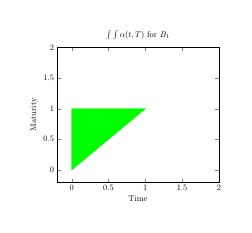
\begin{tikzpicture}[scale = 0.3]
    \begin{axis}[title = {$\int\int\alpha(t,T)$ for $B_1$}, stack plots = y, area style, xlabel = Time, ylabel = Maturity, xmax=2, ymax=2  ]
      \addplot[green] coordinates{(0,0) (1,1)};
      \addplot+[green] coordinates{(0,1) (1,0)} \closedcycle;
    \end{axis}
  \end{tikzpicture}
  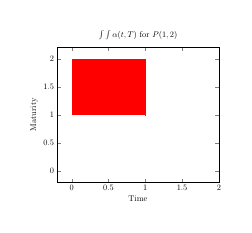
\begin{tikzpicture}[scale = 0.3]
    \begin{axis}[title = {$\int\int\alpha(t,T)$ for $P(1,2)$}, stack plots = y, area style, xlabel = Time, ylabel = Maturity, xmax=2 ]
      \addplot[white] coordinates{(0,0) (1,1) };
      \addplot[white] coordinates{(0,1) (1,0) };
      \addplot+[red] coordinates{(0,1) (1,1) } \closedcycle;
    \end{axis}
  \end{tikzpicture}
  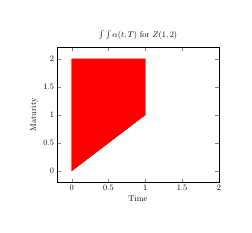
\begin{tikzpicture}[scale = 0.3]
    \begin{axis}[title = {$\int\int\alpha(t,T)$ for $Z(1,2)$}, stack plots = y, area style, xlabel = Time, ylabel = Maturity, xmax=2 ]
      \addplot[red] coordinates{(0,0) (1,1) };
      \addplot+[red] coordinates{(0,2) (1,1) } \closedcycle;
    \end{axis}
  \end{tikzpicture}
\end{frame}
\begin{frame}
  \frametitle{Change of Numeraire}
  Using Ito lemma, we have $dZ(t,T) = Z(t,T) \left( \Sigma(t,T)dW_t + (\frac{1}{2}\Sigma^2(t,T) - \int_t^T \alpha(t,u)du)dt\right)$. Using Girsanov theorem, we have 
  \begin{align*}
    dZ(t,T) &=Z(t,T)\Sigma(t,T)d\tilde{W}_t \\
    \tilde{W}_t &= W_t + \int_0^t \gamma_s ds \\
    \gamma_t &= \frac{1}{2} \Sigma(t,T) - \frac{1}{\Sigma(t,T)}\int_t^T \alpha(t,u) du
  \end{align*}
  Note the $\gamma_s$ is computed from $\alpha(t,T)$ and $\sigma(t,T)$, but cannot not depend on $T$, so this puts restrictions on the functional form of real world drift and vol.
\end{frame}
\begin{frame}
  \frametitle{Rates under $\mathbf{Q}$}
  We should have 0 by differentiate $\gamma$ against $T$, so
  \begin{align*}
    \alpha(t,T) &= \sigma(t,T)( \gamma_t - \Sigma(t,T)) \\
    df(t,T) &= \sigma(t,T)d\tilde{W}_t - \sigma(t,T) \Sigma(t,T)dt \\
    r(t) &= f(0,t) + \int_0^t\sigma(s,t)d\tilde{W}_s - \int_0^t \sigma(s,t) \Sigma(s,t)ds \\
  \end{align*}
  \begin{itemize}
  \item All bonds have to be made into martingale at the same time, so the market is arbitrage free.
  \item Real world drift does not matter, and the vol remains the same. Drift of the bonds goes to 0 not the rates.
  \item Short rate models can be expressed in HJM format ( HW, CIR, BK ) and can have closed form solution. 
  \end{itemize}
\end{frame}
\begin{frame}
  \frametitle{Application to Commodity}
  In commodity, we need to model the forward/futures curve like rates. We know all futures have zero drift.
  \begin{itemize}
  \item Future price equals to forward price, when correlation to margin interest is assumed to be zero.
  \item Forward price process has zero drift.
  \item Forward contract $B_t(F_t-K)$ and futures contract $M_t(F_t-K)$ are both tradables. $B_t$ is usual zcb, while $M_t$ is a money market account that earns risk free interest on the balance.
  \item Forward contract value with zcb as the numeraire $B_t^{-1} B_t F_t$ is a martingale.
  \item Similarly future contract with either $B_t$ or $M_t$ as numeraire $M_t^{-1}M_tF_t$ is also martingale. In fact, ratio of any two tradables' value is a martingale under complete market no arbitrage.
  \end{itemize}
\end{frame}
\begin{frame}
  Assuming a lognormal model for com future, we have 
  $$\frac{dF(t,T)}{F(t,T)}=\sigma(t,T)d\tilde{W}(t)$$
  It is easy to generalize it to 2-factor model: 
  $$\frac{dF(t,T)} { F(t,T)}=\sigma_1(t,T)d\tilde{W}_1(t) + \sigma_2(t,T)d\tilde{W}_2(t)$$
  But good models should be able to both fit/generate realistic scenarios and have parameters that can be controlled with some interpretation. People tends to prefer the model to be specified in a certain way that relates to real world observables (e.g. below Gabillon model), then solve by transform back to a general problem (e.g. Anderson ). 
  $$dF(t,T) = F(t,T)(\sigma_S(t) e^{- \lambda (T - t )} d\tilde{W}_1(t) + \sigma_L d\tilde{W}_2(t))$$
\end{frame}


\end{document}
